\documentclass[../main.tex]{subfiles}
\usepackage[utf8x]{inputenc}
\usepackage{blindtext}
\usepackage{float}
\usepackage{graphicx}
\usepackage{siunitx}
\usepackage{cite}

\begin{document}

Another study takes a look at building efficient HPCs using approximate counting algorithms. Traditionally, one HPC is only set to keep track of one event at execution time, "one-counter-one-event" \cite{memory}. This restriction makes it a bit difficult to collect large data regarding performance, making it necessary to run workloads multiple times to gather that data. This re-running of workloads becomes inefficient and incurs time and resource cost unnecessarily.

Techniques have been introduced to monitor a large number of events using less HPCs, for example, the multiplexing technique. The multiplexing technique, basically, just implies measuring events for a fraction of the execution time and then using that to extrapolate the overall counts, this allows HPCs to be multiplexed and, in turn, cover more events in less amount of runs \cite{memory}. That is not to say that multiplexed counters are accurate rather, the opposite is true with error bounds falling between \(5\% - 30\%\).

Approximate-counting algorithms can be used to improve the accuracy of the HPCs. An approximate-counting algorithm allows the counting of a large number events using a small amount of memory. The counters are incremented based on probability to save memory. Another important algorithm is Morris' Algorithm, which basically uses small data structures in conjunction with simple update algorithms to count the number of events in a stream \cite{memory}.

The Rocket Chip generator is used to realize Morris counters in hardware. The default hardware is a RISC-V in-order pipelined CPU with 29 general 64-bit HPCs and 29 event selector registers. The architecture of the probabilistic HPC is below, provided by \cite{memory}:

\begin{figure}[h]
    \centering
    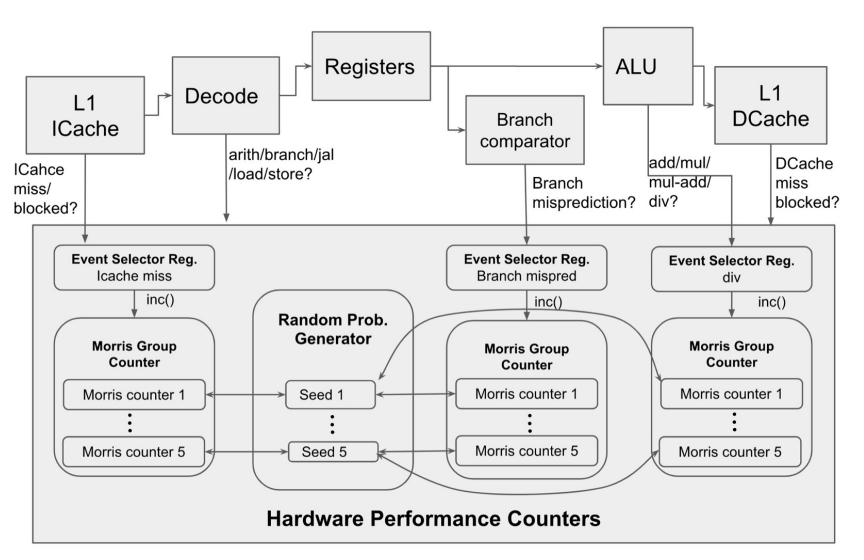
\includegraphics[width=200pt, height=150pt]{contents/images/memory_1.png}
    \caption{Rocket Core with approximate PCs \cite{memory}}
    \label{fig:mem_1}
\end{figure}

A 6-bit Morris counter in which each counter can store \(2^{64}\) counts is used. To combat the large variance of the Morris counters, 5 counters are grouped to form one group...a Morris group counter. All counters in a group count the same event and the average is used \cite{memory}. When compared with the counter that required 64-bits for counting up to \(2^{64}\), the Morris counter achieves that using less than half the bits, leading to a 2x improvement from a storage utilization lens.

The figure below graphs the findings, provided by \cite{memory}:

\begin{figure}[h]
    \centering
    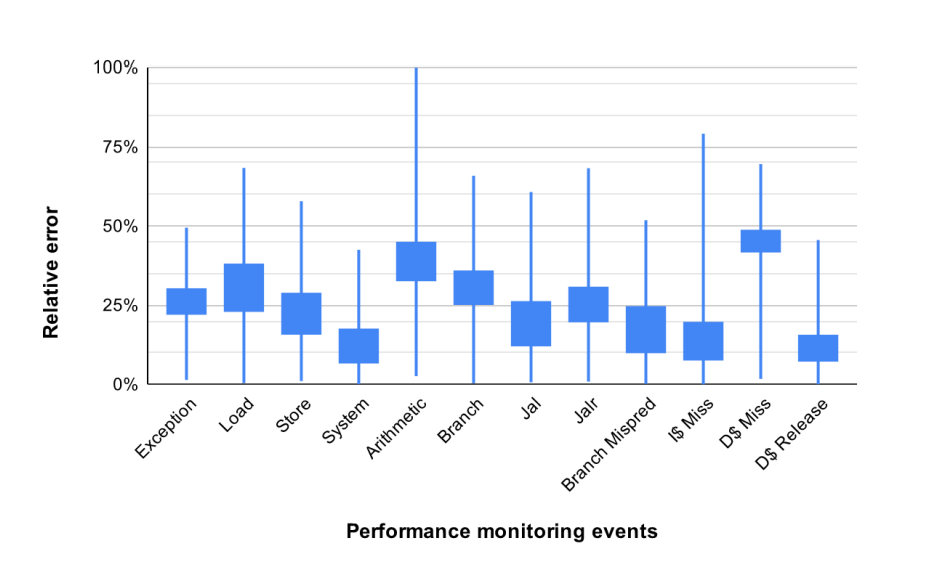
\includegraphics[width=200pt, height=150pt]{contents/images/memory_2.png}
    \caption{Relative Errors of the proposed Approximate Counters \cite{memory}}
    \label{fig:memory_2}
\end{figure}

The graph shows the 3rd quartile, 1st quartile, and the minimum of relative errors for each performance event. It is to be noted that an outlier event was not graphed, an instance where the relative errors for arithmetic was 129\%. The minimum errors stay hovering around 5\% while the maximum errors are absolutely wild, reaching upwards of 120\%. This event is due to the reconstruction performed in the random probability generator module. The module is necessary since the Morris counters rely on randomness to increment the counters \cite{memory}.

Since the HPCs with the approximate counting algorithms use less storage than regular performance counters, nearly half of the bit-width, and show a decrease in relative errors, maybe it's time to switch to using HPCs in tandem with approximate counting algorithms.

\end{document}